\section{Introducci\'on}

En este trabajo resolveremos el problema de encontrar un camino para ir de una a ciudad a otra minimizando el costo del combustible. Para modelar el problema computacionalmente, utilizamos la siguiente representación: tendremos un grafo G, con n nodos y m aristas. Cada nodo representa una ciudad distinta y cada arista una ruta entre dos ciudades. Además cada arista $m_{j}$ tendrá asignado un valor $l_{j}$ que representa la cantidad de litros de nafta que necesita nuestro vehículo para recorrer dicha ruta. Por otro lado, cada nodo $n_{i}$  también tendrá un valor asignado $c_{i}$, que representa el costo de la nafta por litro en dicha ciudad. \\
\indent La capacidad del tanque de nuestro auto será de 60 litros, y nuestro algoritmo devolverá el costo mínimo de combustible partiendo de una ciudad y terminando en otra.\\
\indent Para resolver este problema implementaremos cuatro algoritmos distintos.
\begin{enumerate}
\item Algoritmo de Dijkstra.
\item Algoritmo de Dijkstra con cola de prioridad.
\item Algoritmo de Bellman-Ford.
\item Algoritmo de Floyd-Warshall.
\end{enumerate}

\indent El programa toma como entrada un archivo cuya primera línea debe tener dos enteros $n$ y $m$s correspondientes a la cantidad de ciudades y a la cantidad de rutas respectivamete. Luego habrá n líneas. Cada una con un entero $c_{i}$ que representa el costo del litro de combustible en la ciudad $i$. Luego deberán haber m líneas con tres entero $a_{i}$, $b_{i}$ y $l_{i}$. $a_{i}$ y $b_{i}$ indicarán las ciudades conectadas por la ruta, y $l_{i}$ la cnatidad de litros necesarios para recorrerla. Asumiremos que todos los valores en la entrada serán enteros positivos. Finalmente, el archivo debe tener una línea más. La última línea deberá tener el identificador del método con el que se quiere correr el programa. Los identificadores son los siguientes:
\begin{enumerate}
\item d: Dijkstra.
\item dp: Dijkstra con cola de prioridad.
\item bf: Bellman-Ford.
\item fw: Floyd-Warshall.
\end{enumerate}

\indent La salida, como pide el enunciado, consistirá de $n*(n-1)$ líneas. Cada línea tendrá tres enteros $a_{i}$, $b_{i}$ y $s_{i}$. $a_{i}$ y $b_{i}$ indicarán las ciudades consideradas. $s_{i}$ indicará el costo mínimo para ir por todas las ciudades comenzando en $a_{i}$ y finalizando en $b_{i}$. Las líneas de salida estarán ordenadas según el orden lexicográfico de las ciudades pertinentes. \footnote{Extraído del enunciado.}
Veamos un ejemplo:

\begin{center}
\begin{figure}[H]
\centering
   \begin{minipage}{0.4\textwidth}
     \centering
     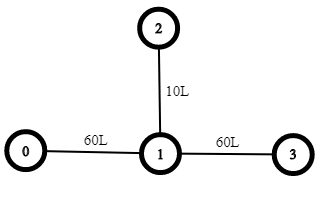
\includegraphics[width=1\linewidth]{img/graph_intro.png}
   \end{minipage}\hfill
\end{figure}
\end{center}

\indent Supongamos que en este caso los costos de combustible para las ciudades 0, 1, 2 y 3 son respectivamente 1, 50, 10, 50. Veamos las distancias de 0 a todos los demas. En primer lugar, tenemos una única forma de llegar al nodo 1, cargando 60L en un total de 60\$. Luego, la distancia de 0 a 1 es 60. Una vez que estamos en 1, tenemos dos opciones. Podemos cargar 10L e ir a 2 (por 500\$), o cargar 60 e ir a 3 (por 3000\$). Notemos que esta no es la mejor estrategia para llegar a 3, ya que podríamos ir a 2, cargar 60L, volver a 1, cargar 10L y de ahí pasar a 3 (por 1600\$). Esto nos resulta en costos totales de 60\$, 560\$ y 1660\$. \\
\indent Sin embargo, notemos que el camino de 0 a 3 resulta ser un camino no simple, lo que imposibilita la utilización de algunos algoritmos de camino mínimo, como Dijkstra. Por este motivo es que la transformación al grafo con 61*n nodos resulta de utilidad, ya que allí, este camino se vuelve simple. Nos permite estar en una misma ciudad más de una vez, pero el estado del tanque será distinto.
